%=========================================================
%  SamplePrograms
%=========================================================
\section{SamplePrograms}
Sample Programs are provided as the projects of Eclipse in the directory "mmRISC-1/workspace". Please import all the projects in the Eclipse Project Explorer in advance.

%=========================================================
\subsection{Integer Instructions: "mmRISC\_SampleCPU"}
First, please build the program and launch a terminal application on Ubuntu, such as the minicom. You can also use the serial terminal windows in the debug perspective of the Eclipse IDE, if you have it. The communication parameters are 115200 bps and 8N1 (8bit, Non-Parity and 1 Stop bit).\\

Before running and debugging the program, change the Eclipse perspective to debug and select the menu of "Run"$\rightarrow$"Debug Configuration". Create a debug configuration "mmRISC\_SampleCPU" in GDB OpenOCD Debugging. Please fill in "./Debug/mmRISC\_SampleCPU.elf" in the C/C++ Application field and click the "Debug" button. The program will break at the beginning of main(). Click the resume button (green right arrow) to restart the program. You can use any debug operations in the Eclipse windows as shown in Figure \ref{fig:ECLIPSEWINDOW}.\\

The MTIME timer requests periodic interrupts to increment the binary number displayed on 10 discrete LEDs. The LED incrementing value is controlled by GPIO2[9:0] and the direction is controlled by GPIO2[10]. Most of GPIO2[9:0] are connected to the slide switches (SW0-SW9) and GPIO2[10] is connected to the push switch (KEY).\\

Additionally, the sample program reads the 3D Acceleration Sensor ADXL345 on the MAX10-Lite board via the I2C interface. It displays some messages and acceleration data in the terminal by using the printf() function.\\

When you type any characters in the terminal, the UART receives each ASCII code and requests a RX interrupt. The software handler for the interrupt displays the code on the left 2-digits of the 7-segment LED and increments a number on the right 4-digits 7-segment LED.\\

The FPGA's operating frequency depends on whether the floating point ISA is implemented or not. Therefore, the program reads the CSR MISA to check if the "F" instruction exists or not and sets the required UART baud rate according to the system clock frequency.

%=========================================================
\subsection{Floating Point Instructions: "mmRISC\_SampleFPU"}
In this Eclipse project property, select "C/C++ Build"$\rightarrow$"Settings"$\rightarrow$"Tool Settings"$\rightarrow$"Target Processor". Then, choose "Single precision extension (RVF)" in the Floating point field and "Single precision (f)" in the Floating point ABI field.\\

This program periodically calculates the floating sinf() functions and displays the results in the serial terminal by using printf() and on the 7-segment LED as a decimal number. During this operation, the periodic MTIME interrupt increments 10 discrete LEDs like in the "mmRISC\_SampleCPU" program.

%=========================================================

\begin{figure}[H]
    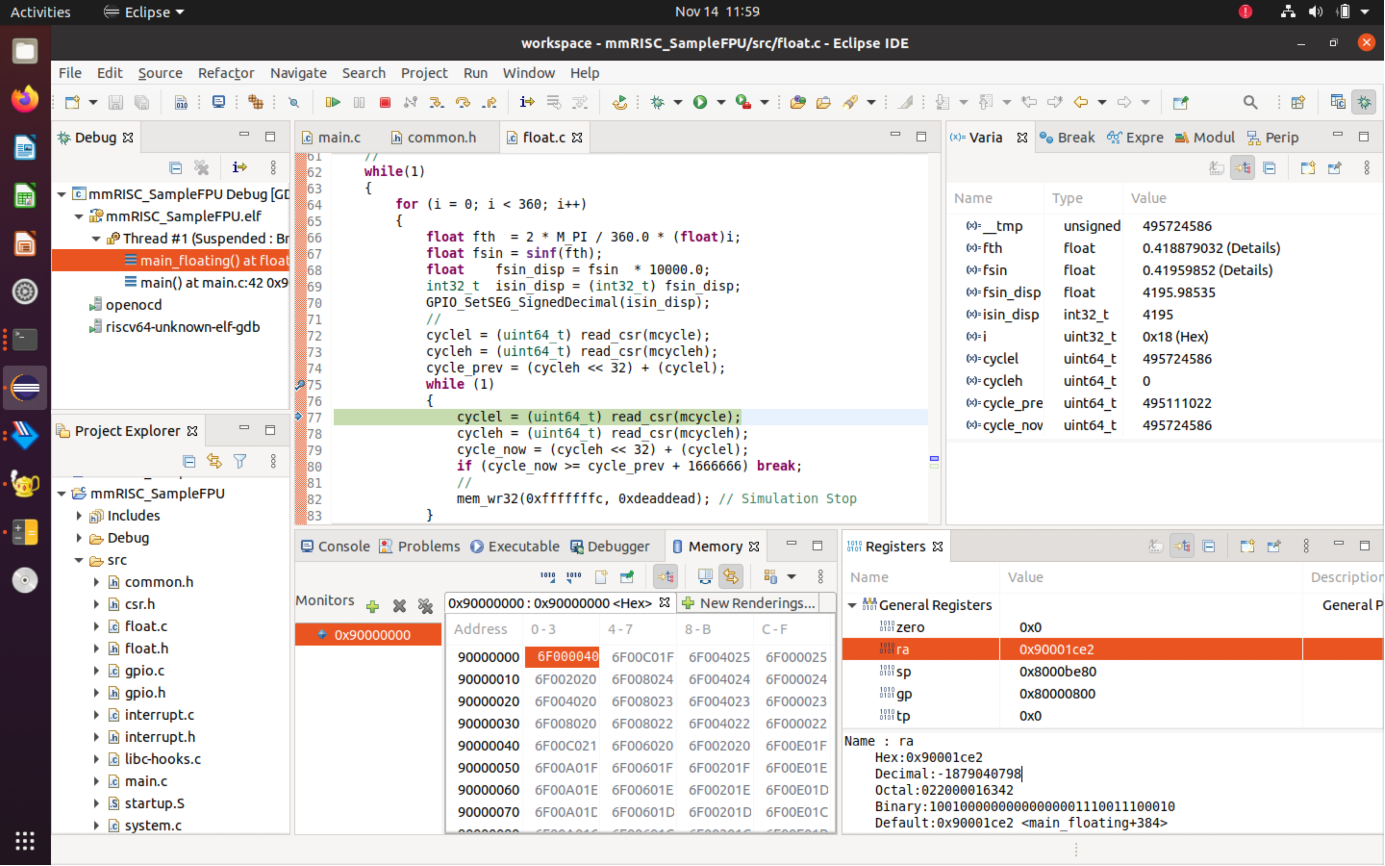
\includegraphics[width=1.0\columnwidth]{./Figure/EclipseWindow.png}
    \caption{Eclipse Windows}
    \label{fig:ECLIPSEWINDOW}
\end{figure}

%=========================================================
\subsection{Integer Instructions: "mmRISC\_Floating"}
This project is a program to verify the Floating Point Operations. Please refer to Section \ref{sec:VERIFYFLOATINGPOINT} for more detailed information.

%=========================================================
\subsection{FreeRTOS Porting "mmRISC\_FreeRTOS"}
This program demonstrates the FreeRTOS porting for mmRISC-1. It implements a typical demo application of the FreeRTOS "Blinky" as a main program. The application sources are in the directory "src\_app" and the RTOS kernel sources are in the directory "src\_kernel". Please launch the terminal window before running this demo.

%=========================================================
\subsection{Dhrystone benchmark "mmRISC\_Dhrystone"}
This is the Dhrystone benchmark program ported to mmRISC-1. Please launch the terminal window before running this benchmark. You will see the benchmark result on it. The calculated scores are shown in Table \ref{tb:BENCHMARKS}.

%=========================================================
\subsection{Coremark benchmark "mmRISC\_Coremark"}
This is the Coremark benchmark program ported to mmRISC-1. Please launch the terminal window before running this benchmark. You will see the benchmark result on it. The calculated scores are shown in Table \ref{tb:BENCHMARKS}.

%=========================================================
\begin{table}[H]
    \begin{adjustbox}{scale={0.9}{1.0}}
    \textsf{
    \begin{tabular}{|L{2cm}{2cm}{t}|L{3cm}{3cm}{t}|L{2cm}{2cm}{t}|L{2.5cm}{2.5cm}{t}|L{2cm}{2cm}{t}|}
        \hline
        %-------------------------------------
        \rowcolor{LightPurple}
        \textbf{Benchmark} &
        \textbf{Compiler} &
        \textbf{Compile Options} &
        \textbf{Result} &
        \textbf{Memory}
        \nextRow \hline
        %-------------------------------------
        \setMultiRow{3}{Dhrystone} &
        riscv64-unknown\lb
        -elf-gcc 10.2.0 &
        -O3 &
        1.55 DMIPS/MHz &
        RAM: \lb
        1cyc R/W
        \nextRow \cline{2-5}
        %-------------------------------------
        ~ &
        riscv64-unknown\lb
        -elf-gcc 10.2.0 &
        -O3 \lb
        -funroll-loops \lb
        -fpeel-loops \lb
        -fgcse-sm \lb
        -fgcse-las \lb
        -flto &
        3.60 DMIPS/MHz &
        RAM: \lb
        1cyc R/W
        \nextRow \cline{2-5}
        %-------------------------------------
        ~ &
        riscv64-unknown\lb
        -elf-gcc 12.2.0 &
        -O3 \lb
        -funroll-loops \lb
        -fpeel-loops \lb
        -fgcse-sm \lb
        -fgcse-las \lb
        -flto &
        3.25 DMIPS/MHz &
        RAM: \lb
        1cyc R/W
        \nextRow \hline
        %-------------------------------------
        \setMultiRow{2}{Coremark} &
        riscv64-unknown\lb
        -elf-gcc 10.2.0 &
        -Ofast \lb
        -funroll-loops \lb
        -fpeel-loops \lb
        -fgcse-sm \lb
        -fgcse-las &
        2.76 Coremark/MHz &
        RAM: \lb
        1cyc R/W
        \nextRow \cline{2-5}
        %-------------------------------------
        ~ &
        riscv64-unknown\lb
        -elf-gcc 12.2.0 &
        -Ofast \lb
        -funroll-loops \lb
        -fpeel-loops \lb
        -fgcse-sm \lb
        -fgcse-las &
        2.51 Coremark/MHz &
        RAM: \lb
        1cyc R/W
        \nextRow \hline
        %-------------------------------------
    \end{tabular}
    }
    \end{adjustbox}
    \caption{Scores of Benchmarks of mmRISC-1 core}
    \label{tb:BENCHMARKS}
\end{table}

%=========================================================
\subsection{A Retro Text Video Game "mmRISC\_StarTrek"}
This is the retro text video game StarTrek. You can play it on the terminal window as shown in Listing \ref{list:STARTREK}. This program is based on "Super Star Trek Classic (v1.1)" ported by Chris Nystrom in 1996.

\begin{lstlisting}[caption=Star Trek Game, label=list:STARTREK, captionpos=b,  language=, frame=single, basicstyle=\ttfamily\scriptsize]

 *************************************
 *                                   *
 *                                   *
 *      * * Super Star Trek * *      *
 *                                   *
 *                                   *
 *************************************

Do you need instructions (y/n): y

...

                         ------*------
         -------------   `---  ------'
         `-------- --'      / /
                  \\-------  --
                  '-----------'

       The USS Enterprise --- NCC - 1701


Your orders are as follows:

   Destroy the 41 Klingon warships which have invaded
 the galaxy before they can attack Federation Headquarters
 on stardate 2641. This gives you 41 days. There is
 1 starbase in the galaxy for resupplying your ship.

Hit any key to accept command. 
Your mission begins with your starship located
in the galactic quadrant Rigel I.

Combat Area  Condition Red
Shields Dangerously Low
------------------------
   <*>          *           Stardate            2600
                            Condition           *RED*
                            Quadrant            2, 1
            +K+             Sector              1, 2
                            Photon Torpedoes    -2013265672
       *                    Total Energy        10
                            Shields             0
                            Klingons Remaining  41
------------------------

Command? 
\end{lstlisting}

%=========================================================
\subsection{A Touch LCD Demo "mmRISC\_TouchLCD"}
The FPGA board DE10-Lite can accommodate the Arduino shield. This demo program supports the following two shields.\\
(1) Adafruit 2.8" TFT Touch Shield for Arduino with Resistive Touch Screen (Product ID 1651); LCD Controller=ILI9341 (SPI I/F), Resistive Touch Controller=STMPE610 (SPI I/F)\\
(2) Adafruit 2.8" TFT Touch Shield for Arduino with Capacitive Touch Screen (Product ID 1947); LCD Controller=ILI9341 (SPI I/F), Capacitive Touch Controller=FT6206 (I2C I/F)

At the early stage of the demo program execution, it checks the existence of the LCD Touch shield and the type of touch controller by accessing the control chip registers. If no LCD Touch shield is found, this demo program toggles LEDs and outputs 3D Acceleration Sensor data to the UART terminal, instead. For the LCD Touch shield with resistive touch, if you press KEY1 at startup, a screen for touch panel calibration will appear. Please touch the center of each small cross section mark that appears on each corner of the LCD screen. For the LCD Touch shield with capacitive touch, calibration is not required.\\
The following graphic routines are prepared in "touchlcd\_tft.c". You can easily understand how to use these functions by reading the source code.
\begin{lstlisting}[language=, basicstyle=\ttfamily\footnotesize]
Pixel          : LCD_Draw_Pixel()
Line           : LCD_Draw_Line()
Rectangle      : LCD_Draw_Rect(),            LCD_Fill_Rect()
Circle         : LCD_Draw_Circle(),          LCD_Fill_Circle()
Circle Quadrant: LCD_Draw_Circle_Quadrant(), LCD_Fill_Circle_Quadrant()
Round Rectangle: LCD_Draw_Round_Rect(),      LCD_Fill_Round_Rect()
Triangle       : LCD_Draw_Triangle(),        LCD_Fill_Triangle()
Text           : LCD_Draw_Char(),            LCD_Draw_String()
Image (BMP)    : LCD_Draw_Image()
\end{lstlisting}

For the image data, you can generate the C source that has the array data from BMP24 by using a perl script mmRISC\_TouchLCD/img/bmp2rgb.pl.\\
Figure \ref{fig:DEMOTOUCHLCD} shows how the demo program works. The image on the top of the screen is generated from ./img/logo.bmp and drawn by LCD\_Draw\_Image(). The strings on the middle of the screen are drawn by LCD\_Draw\_String() and each character is an 8x8 size font defined in ./src/font.h. The bottom-left portion of the screen is a simple painting demo, and the bottom-right portion of the screen shows a bouncing ball controlled by the 3D Acceleration sensor output. This demo supports both panels shown in Figure \ref{fig:TOUCHLCD}.

\begin{figure}[H]
    \includegraphics[width=0.9\columnwidth]{./Figure/DemoTouchLCD.png}
    \caption{Demo Program "mmRISC\_TouchLCD"}
    \label{fig:DEMOTOUCHLCD}
\end{figure}

\begin{figure}[H]
    \includegraphics[width=0.9\columnwidth]{./Figure/TouchLCD.png}
    \caption{Adafruit 2.8" TFT Touch Shield for Arduino (Left: Product ID 1651 Resistive Touch Version; Right: Product ID 1947 Capacitive Touch Version)}
    \label{fig:TOUCHLCD}
\end{figure}

%=========================================================
\subsection{A Touch LCD Demo "mmRISC\_TicTacToe"}
This demo program demonstrates a Tic-Tac-Toe AI game; human vs computer. It also supports the Touch LCD shield of the Arduino, either the Resistive Touch type (Product ID 1651) or the Capacitive Touch type (Product ID 1947). At the early stage of the demo program execution, it checks the existence and the type of the LCD Touch shield by accessing the control chip registers. If the LCD Touch shield is detected, you can play the game on the LCD screen with touch interface as shown in Figure \ref{fig:TICTACTOE1} and Figure \ref{fig:TICTACTOE2}. If the LCD Touch shield is not detected, you can play the game on UART Terminal (8N1, 115200bps) as shown in Listing \ref{list:TICTACTOE}.

\begin{figure}[H]
	\begin{minipage}[t]{0.5\columnwidth}
		\begin{center}
            \includegraphics[width=0.9\columnwidth]{./Figure/TicTacToe(1).png}
		\end{center}
		\caption{Startup Screen of TIc-Tac-Toe Game}
		\label{fig:TICTACTOE1}
	\end{minipage}%
	\begin{minipage}[t]{0.5\columnwidth}
		\begin{center}
            \includegraphics[width=0.9\columnwidth]{./Figure/TicTacToe(2).png}
		\end{center}
		\caption{Ending Screen of TIc-Tac-Toe Game}
		\label{fig:TICTACTOE2}
	\end{minipage}
\end{figure}

\begin{lstlisting}[caption=Tic-Tac-Toe on UART Terminal, label=list:TICTACTOE, captionpos=b,  language=, frame=single, basicstyle=\ttfamily\scriptsize]
=== TictacToe Game ===
1st or 2nd [1-2] ? 1
  ...  (012)
  ...  (345)
  ...  (678)
[You] Move to [0-8] ? 4
  ...  (012)
  .O.  (345)
  ...  (678)
[CPU] Move to 0
  X..  (012)
  .O.  (345)
  ...  (678)

...

[You] Move to [0-8] ? 8
  X.O  (012)
  OOX  (345)
  X.O  (678)
[CPU] Move to 1
  XXO  (012)
  OOX  (345)
  X.O  (678)
[You] Move to [0-8] ? 7
  XXO  (012)
  OOX  (345)
  XOO  (678)
-----------------
---   Draw!   ---
-----------------
\end{lstlisting}
%=========================================================




